%"###############################################
%
% Qmax
%
%###############################################

\subsubsection{Qmax sur 18 mois }

\begin{figure}[H]
\centering
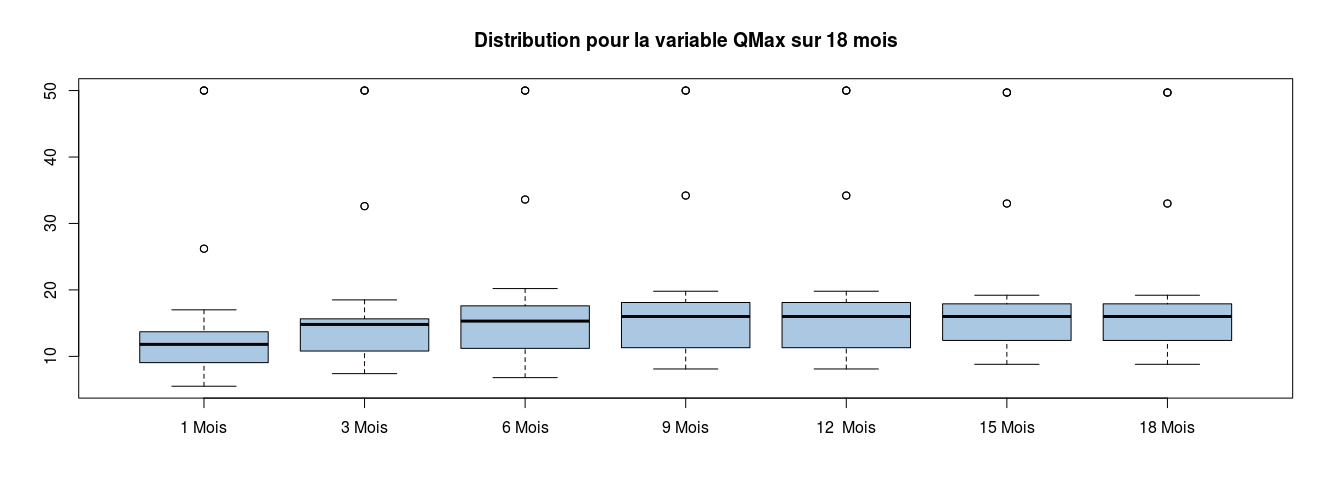
\includegraphics[width=0.75\textwidth]{../Fig/RTUPB/rtupb-boxplot-post-Qmax}
\caption{RTUPB / Qmax sur 18 mois}
\end{figure}	
	
\begin{figure}[H]
\centering
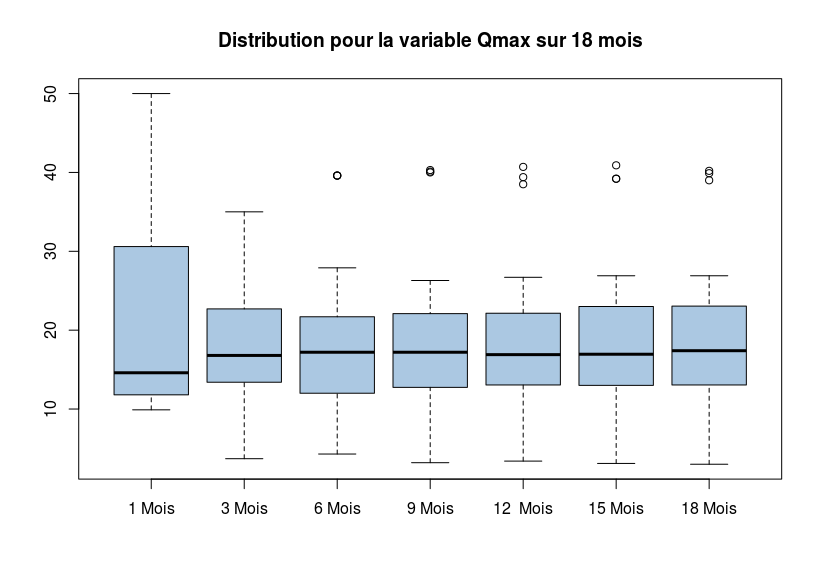
\includegraphics[width=0.75\textwidth]{../Fig/VPPBS/vppbs-boxplot-post-Qmax}
\caption{VPPBS/Qmax sur 18 mois}
\end{figure}


\begin{figure}[H]
\centering
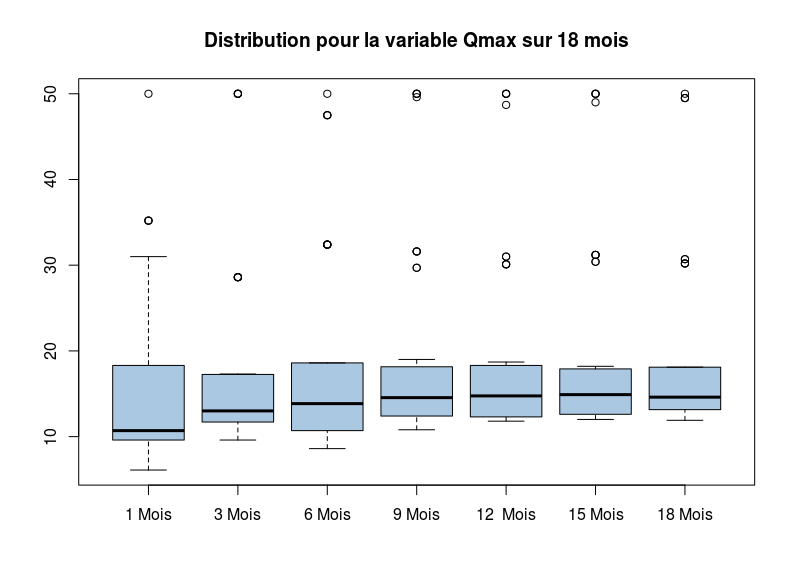
\includegraphics[width=0.75\textwidth]{../Fig/VAPOR/vapor-boxplot-post-Qmax}
\caption{VAPOR/Qmax}
\end{figure}

%
%##########################
%# CONCLUSION
%##########################

RTUPB semble être le plus constant, VPPBS permet d’obtenir de meilleurs résultats sur le Qmax (augmentation) avec des cas extrêmes plus élevés. VAPOR obtient des résultats médians proches de RTUPB mais avec des cas extrêmes plus élevés comparativement aux trois techniques.   